\documentclass{fkssolpub}

\usepackage[czech]{babel}
\usepackage{fontspec}
\usepackage{fkssugar}
\usepackage{amsmath}
\usepackage{graphicx}

\author{Ondřej Sedláček}
\school{Gymnázium Oty Pavla} 
\series{1.3}
\problem{7} 

\begin{document} 

Nechť velikost úhlu $|\angle ACB| = \gamma$ a velikost úhlu $|\angle ACF| = \phi$.
Protože máme zadaný ostroúhlý trojúhelník, prochází výšky trojúhelníku vždy jeho
vnitřkem, proto musí platit $\gamma > \phi$. Pak doplníme zbývající neznámé
úhly:

\begin{figure}[h!]
  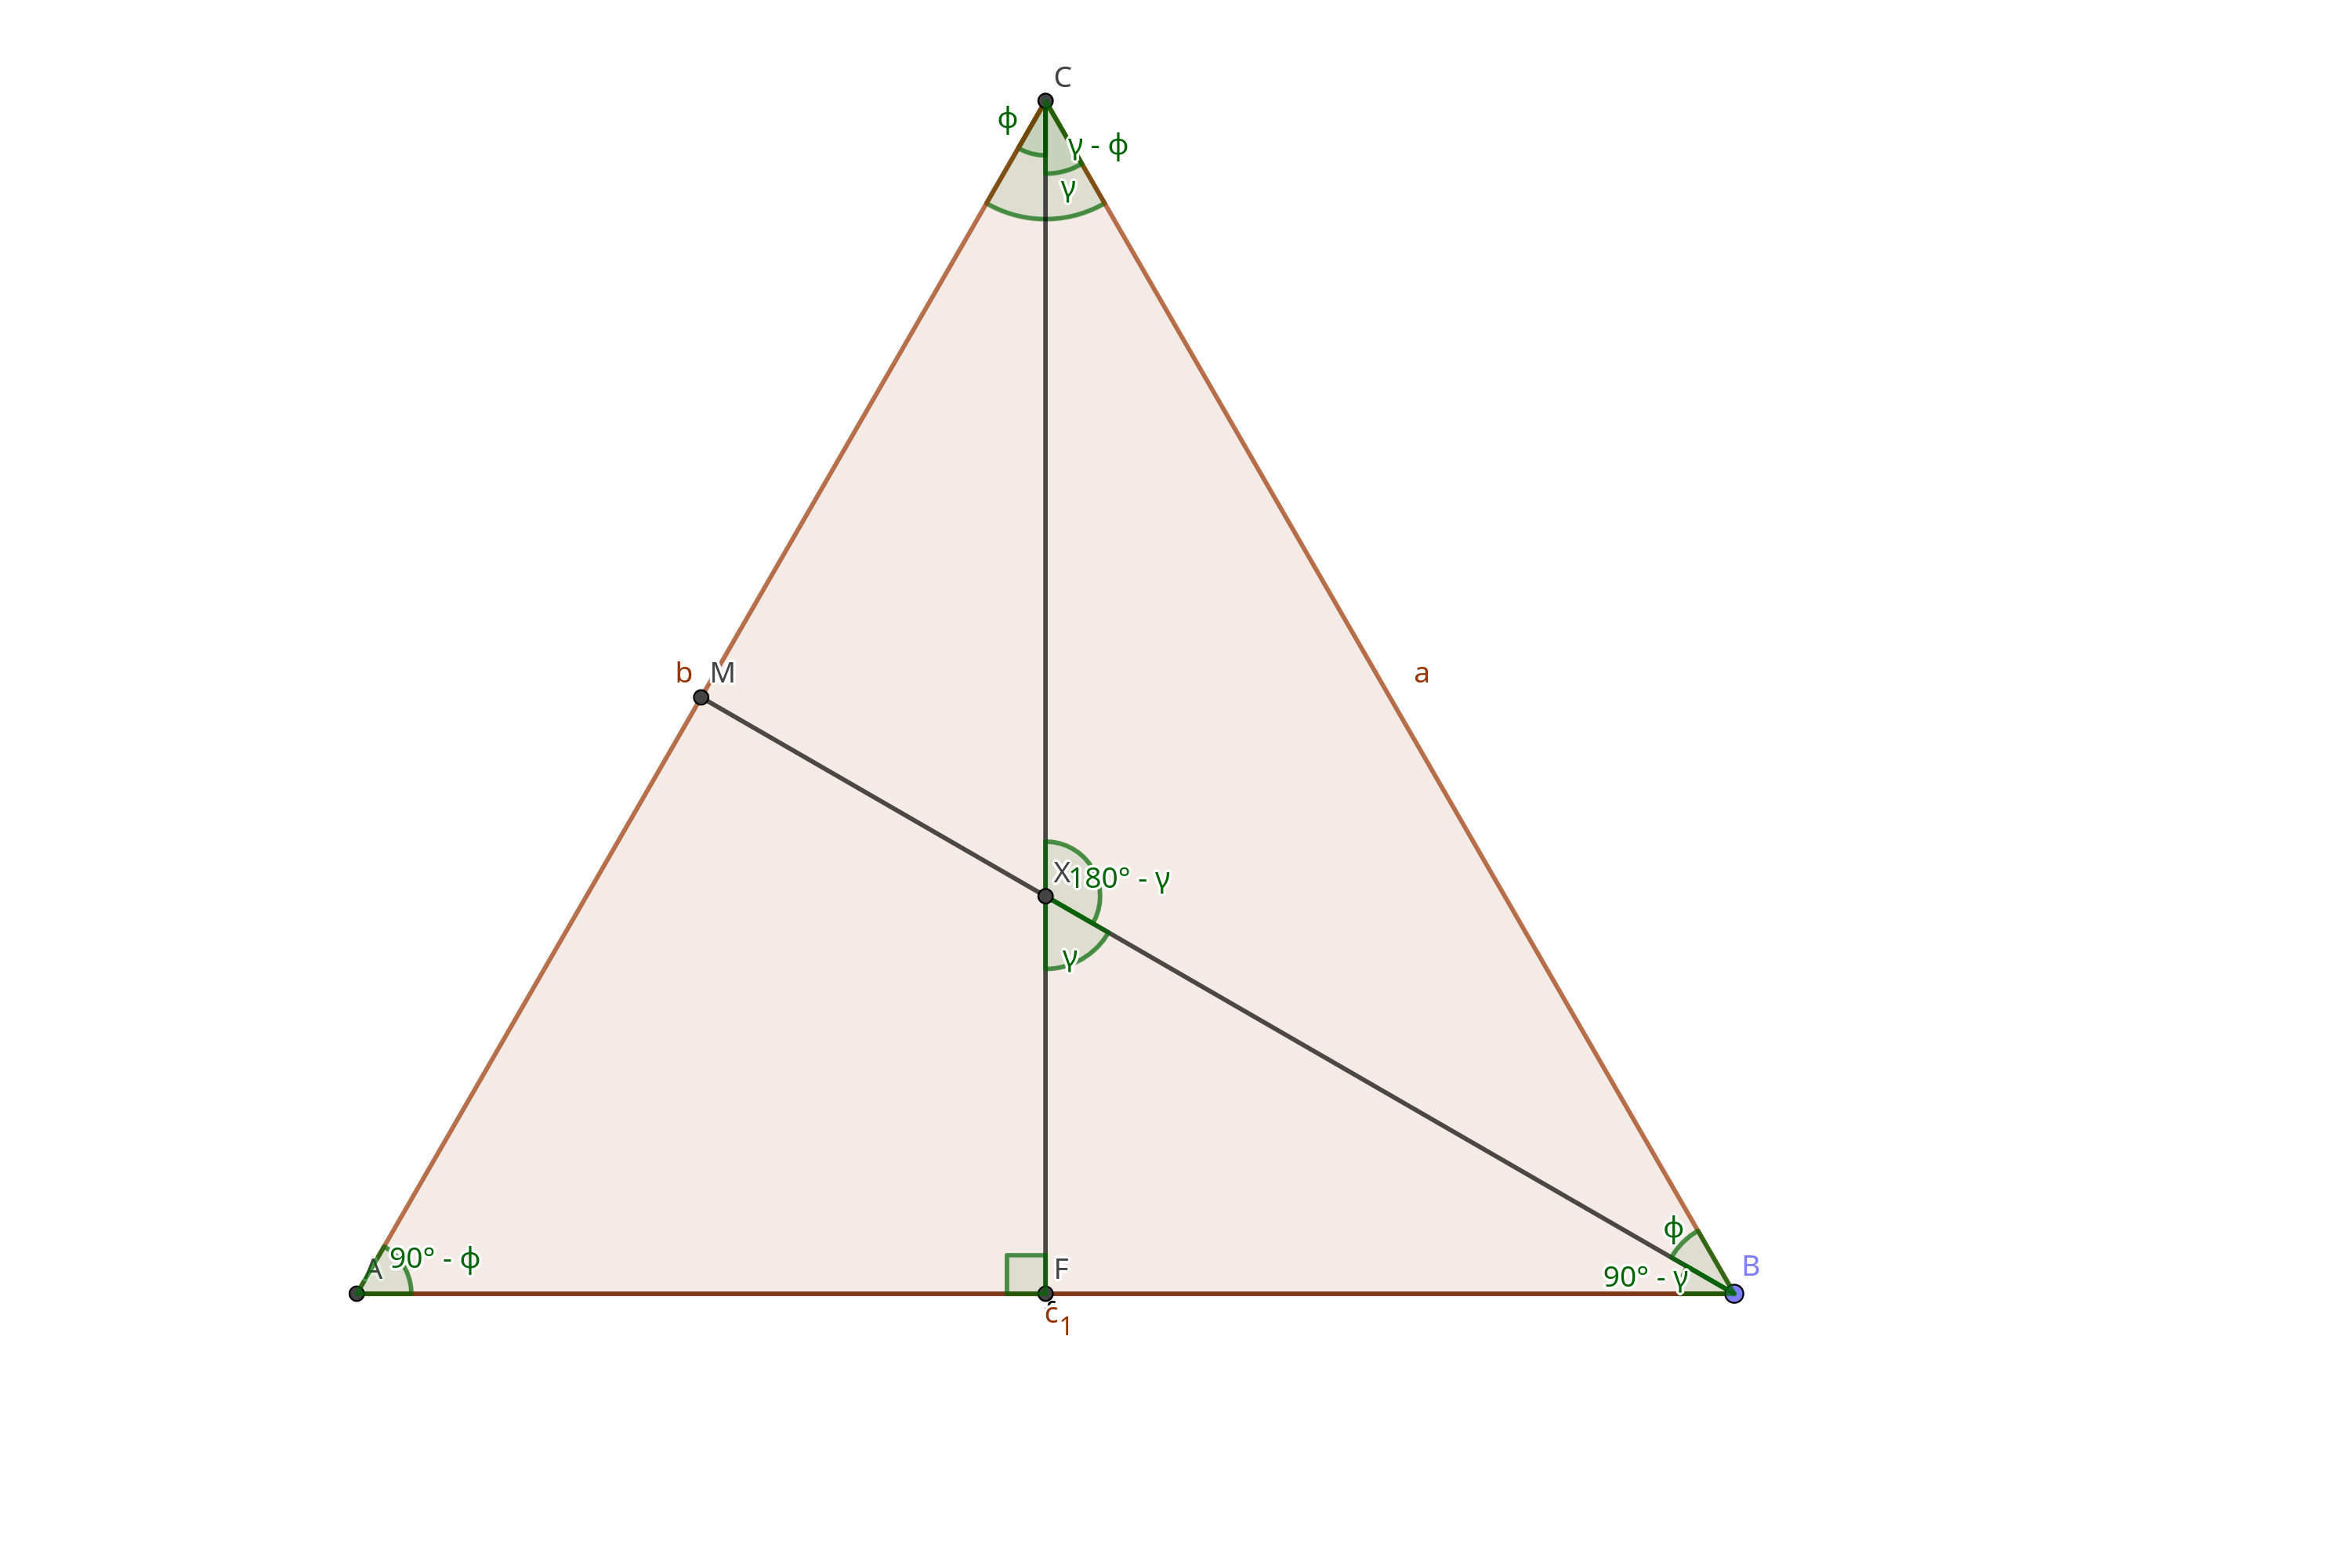
\includegraphics[width=\textwidth]{7-fig.png}
  \caption{Názorný obrázek s dopočítanými úhly}
  \label{fig:1}
\end{figure}

Když doplníme úhly do zadaného trojúhelníku, můžeme si všimnout toho, že pokud
formulujeme sinovou větu pro trojúhelníky $AFC$ a $AMB$, zjistíme, že jeden z poměrů
se musí rovnat:

\[
  \frac{|BM|}{\sin 90^{\circ} - \phi} = \frac{|AM|}{\sin 90^{\circ} - \gamma}
\]
\[
  \frac{|CF|}{\sin 90^{\circ} - \phi} = \frac{|AC|}{\sin 90^{\circ}} = |AC|
\]

Díky čemuž můžeme dostat velikost úhlu $\gamma$:

\[
  \frac{|AM|}{\sin 90^{\circ} - \gamma} = |AC|
\]
\[
  \frac{|AC|}{2 \cdot \cos \gamma} = |AC|
\]
\[
  \cos \gamma = \frac{1}{2}
\]
\[
  \gamma = 60^{\circ}
\]

Když znova formulujeme sinovou větu pro trojúhelníky $AMB$ a $CMB$, dostaneme
soustavu:

\[
  \frac{|BM|}{\sin \gamma} = \frac{|MC|}{\sin \phi}
\]
\[
  \frac{|BM|}{\sin 90^{\circ} - \phi} = \frac{|AM|}{\sin 90^{\circ} - \gamma}
\]

Při vyjádření $|BM|$ z druhé rovnice dostaneme:

\[
  \frac{\frac{|AM| \cdot \cos \phi}{\cos \gamma}}{\sin \gamma} = \frac{|MC|}{\sin \phi}
\]
\[
  \sin \phi \cos \phi = \sin \gamma \cos \gamma
\]
\[
  \sin 2 \phi = \sin 2 \gamma
\]
\[
  \sin 2 \phi = \frac{\sqrt{3}}{2}
\]

Protože musíme splnit podmínku, že $\gamma > \phi$, nemůže $\phi = 60^{\circ}$, proto
jediné řešení této rovnice je $\phi = 30^{\circ}$. 

A protože velikost úhlu $|\angle BAC| = 90^{\circ} - \phi = 60^{\circ}$, trojúhelník
musí být nutně rovnostranný. Q. E. D.

\end{document}
